\subsection{Unet}
U-Net is widely used in image-to-image tasks, e.g. denoising, super-resolution, and segmentation.

\section{Recurrent Neural Network}
\subsection{Sequential Model}

\paragraph{Partial Convolution} Current states only depend on the previous state

\paragraph{Recurrent Neural Network} Introduce hidden state  $ h  $ to stores previous information.

\begin{align*}
    h_t&=f(h_{t-1},x_t)\\
    y_t&=g(h_t)
\end{align*}
recurrent: same  $ f, g  $ for different  $ t $.


\subsubsection{Vanila RNN}
\begin{align*}
    h_t&=\tanh(Wh_{t-1}+Ux_t)\\
    y_t&=Vh_t
\end{align*}

\subsection{Long Short-Term Memory}
Long Short-Term Memory (LSTM) is designed to avoid vanishing or exploding gradients, it is capable of learning long-term dependencies.

For each block, we store a history message.

\name{Cell state}: like a conveyor belt. It runs straight down the entire chain, with only some minor linear interactions. It's very easy for information to just flow along it unchanged.

\name{Gates}: optionally let information through.
\begin{align*}
    \begin{pmatrix}
        i\\
        f\\
        o\\
        \tilde{C}_t
    \end{pmatrix}=\begin{pmatrix}
        \sigma\\
        \sigma\\
        \sigma\\
        \tanh
    \end{pmatrix}\begin{pmatrix}
        W_i\\
        W_f\\
        W_o\\
        W_c
    \end{pmatrix}\begin{pmatrix}
        h_{t-1}\\
        x_t
    \end{pmatrix}
\end{align*}
\[C_t=f_t\odot C_{t-1}+i_t\odot \tilde{C}_t\]
\[h_t=o_t\odot \tanh(C_t)\]

Input gate  $ i $, forget gate  $ f:f_t=1 $ and output gate  $ o $. 

Gate  $ i,f,o $ control the information flow.

It gives the information flow  $ h $ and the history memory flow  $ C $. So it can go deeper.

\begin{figure}[htbp]
    \centering
    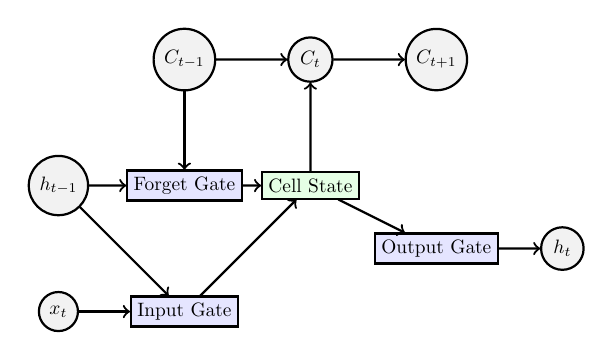
\begin{tikzpicture}[thick,scale=0.8, every node/.style={scale=0.7}]
        % Gates
        \node[draw, rectangle, fill=blue!10, minimum width=0.6cm, minimum height=0.4cm] (forget_gate) at (0, 2) {Forget Gate};
        \node[draw, rectangle, fill=blue!10, minimum width=0.6cm, minimum height=0.4cm] (input_gate) at (0, 0) {Input Gate};
        \node[draw, rectangle, fill=blue!10, minimum width=0.6cm, minimum height=0.4cm] (output_gate) at (4, 1) {Output Gate};
        
        % Cell state
        \node[draw, rectangle, fill=green!10, minimum width=0.6cm, minimum height=0.4cm] (cell_state) at (2, 2) {Cell State};
        
        % Input and hidden state
        \node[draw, circle, fill=gray!10, minimum size=0.4cm] (input) at (-2, 0) {$x_t$};
        \node[draw, circle, fill=gray!10, minimum size=0.4cm] (hidden_prev) at (-2, 2) {$h_{t-1}$};
        
        % Outputs
        \node[draw, circle, fill=gray!10, minimum size=0.4cm] (hidden_next) at (6, 1) {$h_t$};
        \node[draw, circle, fill=gray!10, minimum size=0.4cm] (cell_next) at (2, 4) {$C_t$};
        \node[draw, circle, fill=gray!10, minimum size=0.4cm] (cell_prev) at (0, 4) {$C_{t-1}$};
        \node[draw, circle, fill=gray!10, minimum size=0.4cm] (cell_future) at (4, 4) {$C_{t+1}$};
        
        % Connections
        \draw[->] (input) -- (input_gate);
        \draw[->] (hidden_prev) -- (forget_gate);
        \draw[->] (hidden_prev) -- (input_gate);
        \draw[->] (forget_gate) -- (cell_state);
        \draw[->] (input_gate) -- (cell_state);
        \draw[->] (cell_prev) -- (forget_gate);
        \draw[->] (cell_prev) -- (cell_next);
        \draw[->] (cell_state) -- (cell_next);
        \draw[->] (cell_next) -- (cell_future);
        \draw[->] (cell_state) -- (output_gate);
        \draw[->] (output_gate) -- (hidden_next);
    \end{tikzpicture}
    \caption{Single LSTM Cell Structure with Extended Cell State Flow}
    \label{fig:single_lstm_extended}
\end{figure}

\begin{figure}[htbp]
    \centering
    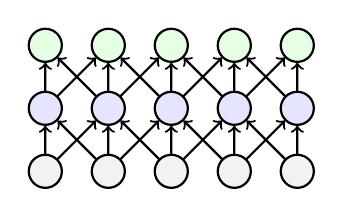
\begin{tikzpicture}[thick,scale=0.8, every node/.style={scale=0.7}]
        % Input layer
        \foreach \i in {1,...,5} {
            \node[draw, circle, fill=gray!10, minimum size=0.6cm] (input\i) at (\i, 0) {};
        }
        
        % Hidden layer
        \foreach \i in {1,...,5} {
            \node[draw, circle, fill=blue!10, minimum size=0.6cm] (hidden\i) at (\i, 1) {};
        }
        
        % Output layer
        \foreach \i in {1,...,5} {
            \node[draw, circle, fill=green!10, minimum size=0.6cm] (output\i) at (\i, 2) {};
        }
        
        % Connections
        \foreach \i in {1,...,5} {
            \foreach \j in {1,...,5} {
                \ifnum \j=\i
                    \draw[->] (input\i) -- (hidden\j);
                \else
                    \ifnum \j=\numexpr\i-1\relax
                        \draw[->] (input\i) -- (hidden\j);
                    \else
                        \ifnum \j=\numexpr\i+1\relax
                            \draw[->] (input\i) -- (hidden\j);
                        \fi
                    \fi
                \fi
            }
        }
        
        \foreach \i in {1,...,5} {
            \foreach \j in {1,...,5} {
                \ifnum \j=\i
                    \draw[->] (hidden\i) -- (output\j);
                \else
                    \ifnum \j=\numexpr\i-1\relax
                        \draw[->] (hidden\i) -- (output\j);
                    \else
                        \ifnum \j=\numexpr\i+1\relax
                            \draw[->] (hidden\i) -- (output\j);
                        \fi
                    \fi
                \fi
            }
        }
    \end{tikzpicture}
    \caption{CNN Networks}
    \label{fig:cnn_restricted}
\end{figure}

\begin{figure}[htbp]
    \centering
    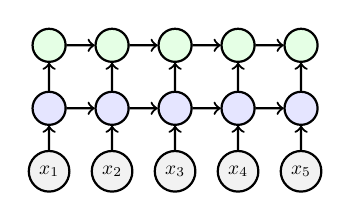
\begin{tikzpicture}[thick,scale=0.8, every node/.style={scale=0.7}]
        % Input layer
        \foreach \i in {1,...,5} {
            \node[draw, circle, fill=gray!10, minimum size=0.6cm] (input\i) at (\i, 0) {$x_\i$};
        }
        
        % Hidden layer
        \foreach \i in {1,...,5} {
            \node[draw, circle, fill=blue!10, minimum size=0.6cm] (hidden\i) at (\i, 1) {};
        }
        
        % Output layer
        \foreach \i in {1,...,5} {
            \node[draw, circle, fill=green!10, minimum size=0.6cm] (output\i) at (\i, 2) {};
        }
        
        % Connections from input to hidden
        \foreach \i in {1,...,5} {
            \draw[->] (input\i) -- (hidden\i);
        }
        
        % Connections within hidden layer
        \foreach \i in {1,...,4} {
            \pgfmathtruncatemacro{\j}{\i+1}
            \draw[->] (hidden\i) -- (hidden\j);
        }
        
        % Connections from hidden to output
        \foreach \i in {1,...,5} {
            \draw[->] (hidden\i) -- (output\i);
        }
        
        % Connections within output layer
        \foreach \i in {1,...,4} {
            \pgfmathtruncatemacro{\j}{\i+1}
            \draw[->] (output\i) -- (output\j);
        }
    \end{tikzpicture}
    \caption{RNN Network}
    \label{fig:rnn_network}
\end{figure}

\section{Transformer}
\subsection{Vision Attention}
\paragraph{V1(Primary Visual Cortex)} V1 is the first stage of visual processing in the brain. It is responsible for processing basic visual features (edges, orientation)
\paragraph{V1 Saliency Hypothesis} V1 transforms the visual inputs into a saliency map of the visual field to guide visual attention of direction of gaze.

\subsection{Context Attention}
One word "attends" to other words in the same sentence differently.

Context information in different sentence is not of fixed length.


\subsection{Attention}
\name{Attention} in deep learning is a vector of importance weight.

Automatically search for parts of a source sentence that are relevant to predicting a target word.

Attention:
\begin{enumerate}
    \item query-key matching
    \[s_i=q_i\cdot k_i\]
    \item compute weights(attention)
    \[ w_i=\mathrm{softmax}(s_i)\]
    \item weighted averaging 
    \[z\sum_{i}w_iv_i\]
\end{enumerate}
\begin{figure}[htbp]
    \centering
    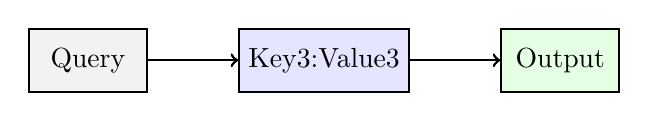
\begin{tikzpicture}[node distance=3cm, auto, thick]
        % Nodes
        \node[draw, rectangle, fill=gray!10, minimum width=1.5cm, minimum height=0.8cm] (query) {Query};
        \node[draw, rectangle, fill=blue!10, minimum width=1.5cm, minimum height=0.8cm, right of=query] (key1) {Key1:Value1};
        \node[draw, rectangle, fill=blue!10, minimum width=1.5cm, minimum height=0.8cm, right of=query] (key2) {Key2:Value2};
        \node[draw, rectangle, fill=blue!10, minimum width=1.5cm, minimum height=0.8cm, right of=query] (key3) {Key3:Value3};
        \node[draw, rectangle, fill=green!10, minimum width=1.5cm, minimum height=0.8cm, right of=key3] (output) {Output};
        
        % Arrows
        \draw[->] (query) -- (key1);
        \draw[->] (query) -- (key2);
        \draw[->] (query) -- (key3);
        \draw[->] (key1) -- (output);
        \draw[->] (key2) -- (output);
        \draw[->] (key3) -- (output);
    \end{tikzpicture}
    \caption{Query $\rightarrow$ Key:Value $\rightarrow$ Output}
    \label{fig:linked_list}
\end{figure}

For multiple queries 
\begin{enumerate}
    \item query-key matching
    \[S=QK^T\]
    \item compute weights(attention)
    \[W=\mathrm{softmax}(\frac{S}{\sqrt{c}})\]
    For independent  $ q_i,k_i  $, with mean  $ 0  $ and variance  $ q $,  scaled dot=product also has mean  $ 0  $ and variance  $ 1 $. 
    \item weighted averaging 
    \[Z=WV\]
\end{enumerate}
where the queries are a   $ q\times c $ matrix and keys are a   $ k\times c $ matrix. And values are  $ k\times d $ matrix and output are $ q\times d $ matrix.

Input  $ X=(x_t)_t $:
\begin{itemize}
    \item Long Context: compute attention across the whole sequence.
    \item Weight  $ W_q,Q_k,Q_v $  are shared by all  $ X_t $.
    \[\begin{aligned}
        Q_t&=X_tW_q\in \Rbb^{n\times m}\\
        K_t&=X_tW_k\in \Rbb^{n\times m}\\
        V_t&=X_tW_v\in \Rbb^{n\times d}
    \end{aligned}\]
\end{itemize}
It gives the outputs, which can be as the input of another attention block.

And we can define different heads (like channels in CNN) extract different information.